\documentclass{elsarticle}

\usepackage{amsmath}
\usepackage{algorithm}
\usepackage{algpseudocode}
\usepackage{minted}
\usepackage{xcolor}

\begin{document}

\begin{frontmatter}
\author{Ashwin Srinath}
\title{A}
\maketitle

\begin{abstract}

\end{abstract}

\end{frontmatter}

%----------------------------------------------------------------------%
    
\section{Introduction}

The solution of a tridiagonal system
for several different right hand sides
appears in several numerical schemes
in Computational Fluid Dynamics (CFD)
such as
compact finite differences \cite{lele1992compact},
Alternating Direction Implicit (ADI) methods \cite{1955ADI}, and
numerical solutions to one-dimensional differential equations.
In such applications,
the evaluation of the tridiagonal systems constitutes
a significant portion of the runtime.
Recently, there has been considerable interest in the CFD community
in developing tridiagonal solvers that
exploit the massive parallelism afforded by
Graphics Processing Units (GPUs)
to speed up the computations
\cite{tutkun2012gpu}
\cite{esfahanian2014efficient}
\cite{GoSt11CR}.
The performance of tridiagonal solvers on the GPU
has been shown to depend on several factors,
such as
choice of algorithm and the associated complexity,
thread utilization,
use of the available memory heirarchy,
and synchronization and control costs
\cite{Zhang2010FTS}.
Many approaches described in the literature
seek to make tradeoffs between these factors
to arrive at a solver that best fits the requirements.
But to our knowledge,
the algorithms proposed so far
are applicable to general tridiagonal systems,
and make no attempt to take advantage of
the known structure of the tridiagonal matrix.

For the relatively common case of structured grids
with constant spacing in each coordinate direction,
the above schemes lead to tridiagonal systems with
\emph{near-Toeplitz} structure
We describe the implementation of a GPU solver that
uses this information to
reduce the number of computations
and access memory more efficiently.
The resulting solver is thus able to perform twice as fast as
the equivalent NVIDIA CUSPARSE solver,
and an Intel MKL solver running with 16 independent cores.

This paper is organized as follows:
Section \ref{sec:preliminaries}
describes algorithms for solving tridiagonal systems on GPUs.
The cyclic reduction algorithm in particular, is discussed in detail,
and issues with its implementation on GPUs is discussed.
Section \ref{sec:proposed-algorithm}
describes our proposed solver for near-Toeplitz tridiagonal systems.
Section \ref{sec:results-single-gpu}
provides an overview of the performance of our solver,
and compares it with other implementations.

%----------------------------------------------------------------------%
\section{Preliminaries} \label{sec:preliminaries}

\subsection{Cyclic reduction}

\begin{equation} \label{eqn:general-tridiagonal-system}
\begin{pmatrix}
     b_1 & c_1  \\
     a_2 & b_2  &  c_2  \\
         & a_3  &  b_3 &  c_3  \\
         &      &  a_4 &  b_4 &  c_4  \\
         &      &      &      &  \ddots \\
         &      &      &      &     &  \ddots  \\
         &      &      &      &     &  a_n  &  b_n
\end{pmatrix}
\begin{bmatrix}
    x_1 \\
    x_2 \\
    x_3 \\
    x_4 \\
    \vdots \\
    \vdots \\
    x_n
 \end{bmatrix}
=
\begin{bmatrix}
   d_1 \\
   d_2 \\
   d_3 \\
   d_4 \\
   \vdots \\
   \vdots \\
   d_{n}
\end{bmatrix}
\end{equation}

Cyclic reduction is applicable to the solution of
general tridiagonal systems of the form
(\ref{eqn:general-tridiagonal-system}).
The algorithm consists of two phases:
\emph{forward reduction} and \emph{backward substitution}.
In the forward reduction phase,
every even-indexed equation $i$
is expressed as a
linear combination of equations $i$, $i-1$ and $i+1$,
yielding a new tridiagonal system of
$n/2$ equations in $n/2$ unknowns
(Equations \ref{eqn:forward-reduction-1} - \ref{eqn:forward-reduction-4}).
The process is repeated until a system of
2 equations in 2 unknowns is left.

\begin{align} 
& a^{\prime}_i = -a_{i-1}k_1 \
    \label{eqn:forward-reduction-1}& \\
& b^{\prime}_i = b_i - c_{i-1}k_1 - a_{i+1}k_2 \
    \label{eqn:forward-reduction-2}& \\
& c^{\prime}_i = -c_{i+1}k_2 \
    \label{eqn:forward-reduction-3}& \\
& d^{\prime}_i = d_i - d_{i-1}k_1  - d_{i+1}k_2 \
    \label{eqn:forward-reduction-4}&
\end{align}

where,

\begin{equation*}
k_1 = \frac{a_i}{b_{i-1}},
k_2 = \frac{c_i}{b_{i+1}}
\end{equation*}

The 2-by-2 system of equations is solved trivially,
yielding $x_n$ and $x_{n/2}$.
In the backward substitution phase,
every odd-indexed unknown $x_i$ is solved for by
substituting the known values of $x_{i-1}$ and $x_{i+1}$
(Equation \ref{eqn:back-substitution}) .

\begin{align} \label{eqn:back-substitution}
x_i = \frac{d^{\prime}_i - a^{\prime}_ix_{i-1} - \
    c^{\prime}_ix_{i+1}}{b^{\prime}_i}
\end{align}

For the last index $i=n$,
the forward reduction step is instead:
\begin{align} \label{eqn:forward-reduction-last}
    & a^{\prime}_n = -a_{n-1}k_1 & \\
    & b^{\prime}_n = b_n - c_{n-1}k_1 & \\
    & d^{\prime}_n = d_n - d_{n-1}k_1&
\end{align}

And for $i=1$, the backward substitution step is instead:
\begin{align} \label{eqn:back-substitution-first}
x_1 = \frac{d^{\prime}_1 - c^{\prime}_1x_{2}}{b^{\prime}_1}
\end{align}

Thus, in the best case ($n$ parallel processors),
cyclic reduction requires 
$2log(n) - 1$ steps.
For even moderately large $n$,
this is significantly smaller than
the $2n$ steps required by the classical Thomas algorithm.
This makes cyclic reduction a good fit
for massively parallel architectures like GPUs.

\begin{figure}[h!]
\begin{center}
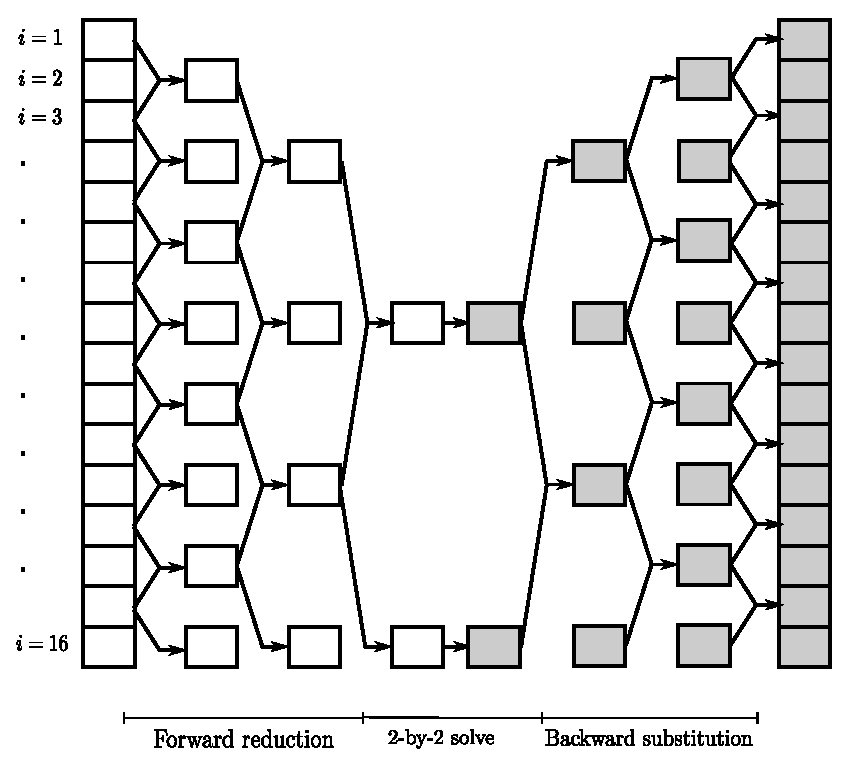
\includegraphics[height=200pt]{img/cyclic-reduction.eps}
\end{center}
\caption{Cyclic reduction - the highlighted elements
show the order in which values are solved for}
\label{fig:cyclic-reduction}
\end{figure}

\subsection{GPU architecture} \label{sec:gpu-architecture}

Writing applications that effectively exploit the GPU
requires a thorough understanding of the underlying architecure.
We provide the pertinent details here,
and refer to \cite{GPUcomputingera} for a more complete picture.
Our tests are performed on the NVIDIA Tesla K20 and K40 GPUs,
built on the ``Kepler'' architecture,
an overview of which is available at \cite{Keplerwhitepaper}.

Applications that use the GPU include special
pieces of code that are executed on the GPU,
referred to as \emph{kernels}.
In C, for example, kernels are written as functions,
and are called with (almost) the same conventions.
A kernel is executed in parallel by several threads,
which are organized into a \emph{grid} of \emph{thread blocks}
(or just \emph{blocks}).
As a requirement, thread blocks must be able to run
independent of each other,
in series or in parallel.

From the hardware perspective, an NVIDIA GPU may be viewed primarily as
a collection of so-called Streaming Microprocessors (SMs).
When a kernel is launched (with a specified number of thread blocks),
each block is assigned to an SM.
Threads within a thread block can execute concurrently on the SM,
and an SM can execute several thread blocks concurrently.
The number of thread blocks that an SM can execute concurrently
is limited by a number of factors,
and maximizing this number is often key to obtaining good performance.

Every thread in every block has access to so-called \emph{global memory},
which can also be accessed by the CPU (or \emph{host}) via the PCI-e bus.
Further,
threads within a thread block have access
to a common, fast, limited \emph{shared memory}.
The contents of shared memory are managed by the kernel code,
and shared memory is often viewed as an explicitly controlled cache.
Each thread also has private \emph{local memory},
and access to extremely fast registers.
Unlike CPUs, the GPU has a large number of registers---a
thread executing a kernel will
typically attempt to store the variables defined in registers,
before spilling over to local memory, which is much slower.

Thread access to global memory is slow,
and is especially inefficient when
successive threads in a block
access locations that are far apart in memory---known
as \emph{uncoalesced} memory access.
Shared memory access can be expected to be
much faster than global memory---however,
the amount of shared memory per SM is limited
(48 KiB for current GPUs).
The amount of shared memory actually used by each block,
can thus limit the number of blocks that
concurrently run on each SM---known as the \emph{occupancy}.
The number of registers per SM is also limited,
and the use of registers can similarly affect occupancy.
Finally, memory transfers between the CPU (host) and GPU (device)
are extremely expensive, limited by the bandwidth of the PCI-e bus.

\subsection{Cyclic reduction implementation on GPU}

As shown in Figure \ref{fig:cyclic-reduction},
in the forward reduction phase,
elements are accessed in a \emph{strided} fashion.
At every subsequent step,
this stride is doubled, while the number of active threads is halved.
In the backward substitution phase,
the strides are halved at each step,
while the number of active threads is doubled.

Before any computations begin,
The coefficient arrays $a$, $b$, $c$
and right-hand sides $d_k$
for all tridiagonal systems $k$
reside in global memory---the
traditional approach is store these right hand sides in
a contiguous buffer.

\subsubsection{Global memory}

The advantage of a global memory implementation is that
threads are constantly busy

\subsubsection{Shared memory}



are stored in global memory,
the large strides in the later stages of forward reduction
and the earlier stages of backward substitution
(Figure \ref{fig:cyclic-reduction})
introduce the problem of uncoalesced memory access.

To overcome this limitation,
each block loads its system to shared memory,
and writes the result back to the appropriate location in
global memory.
The limited amount of shared memory places restrictions
on the size of tridiagonal systems that can be solved.
Shared memory usage is also associated with
lowered GPU occupancy (Section \ref{sec:gpu-architecture}.
Further, as described by Zhang et al.,
the memory access pattern in
cyclic reduction involves \emph{bank conflicts},
leading to performance penalties.
Zhang et al. \cite{Zhang2010FTS} propose a
\emph{hybrid} solver
that uses both cyclic reduction and parallal cyclic reduction
to reduce bank conflicts.
G{\"o}dekke et al. \cite{GoSt11CR}
present an approach that is free of bank conflicts,
but uses additional shared memory.
Davidson et al. describe the method of \emph{register packing}
as a means to reduce shared memory usage in
downsweep-upsweep patterns.
This approach launches fewer threads,
with each thread computing several elements,
and working with registers rather than shared memory.
The above approaches are applicable 


%----------------------------------------------------------------------%
\section{Proposed algorithm} \label{sec:proposed-algorithm}

We note that solving the equations
\ref{eqn:forward-reduction-1}-\ref{eqn:forward-reduction-3}
for each grid line and at each time step of the simulation
is wasteful.
It may be benefitial to
\emph{precompute} and store the coefficients appearing at
each step of the forward reduction,
and to load these values from memory when required.

\subsection{General tridiagonal matrix}

For a general tridiagonal matrix,
in addition to the $3n$ original coefficient arrays
$a$, $b$ and $c$,
this requires extra storage of 
$\frac{n}{2}+\frac{n}{4}+\frac{n}{8}+...=n$
elements each
for $a_i$, $b_i$, $c_i$, $k_{1,i}$ and $k_{2,i}$
appearing at the forward reduction steps.
This additional storage cost is greatly amortized
when solving the same system for multiple right-hand sides.
But the additional arrays
still need to be loaded into shared memory for each thread block.
This raises the shared memory storage from $4n$ to $9n$,
which significantly impacts the number of
concurrently running blocks.

\subsection{Near-Toeplitz matrix}

\begin{figure}[h!]
\begin{center}
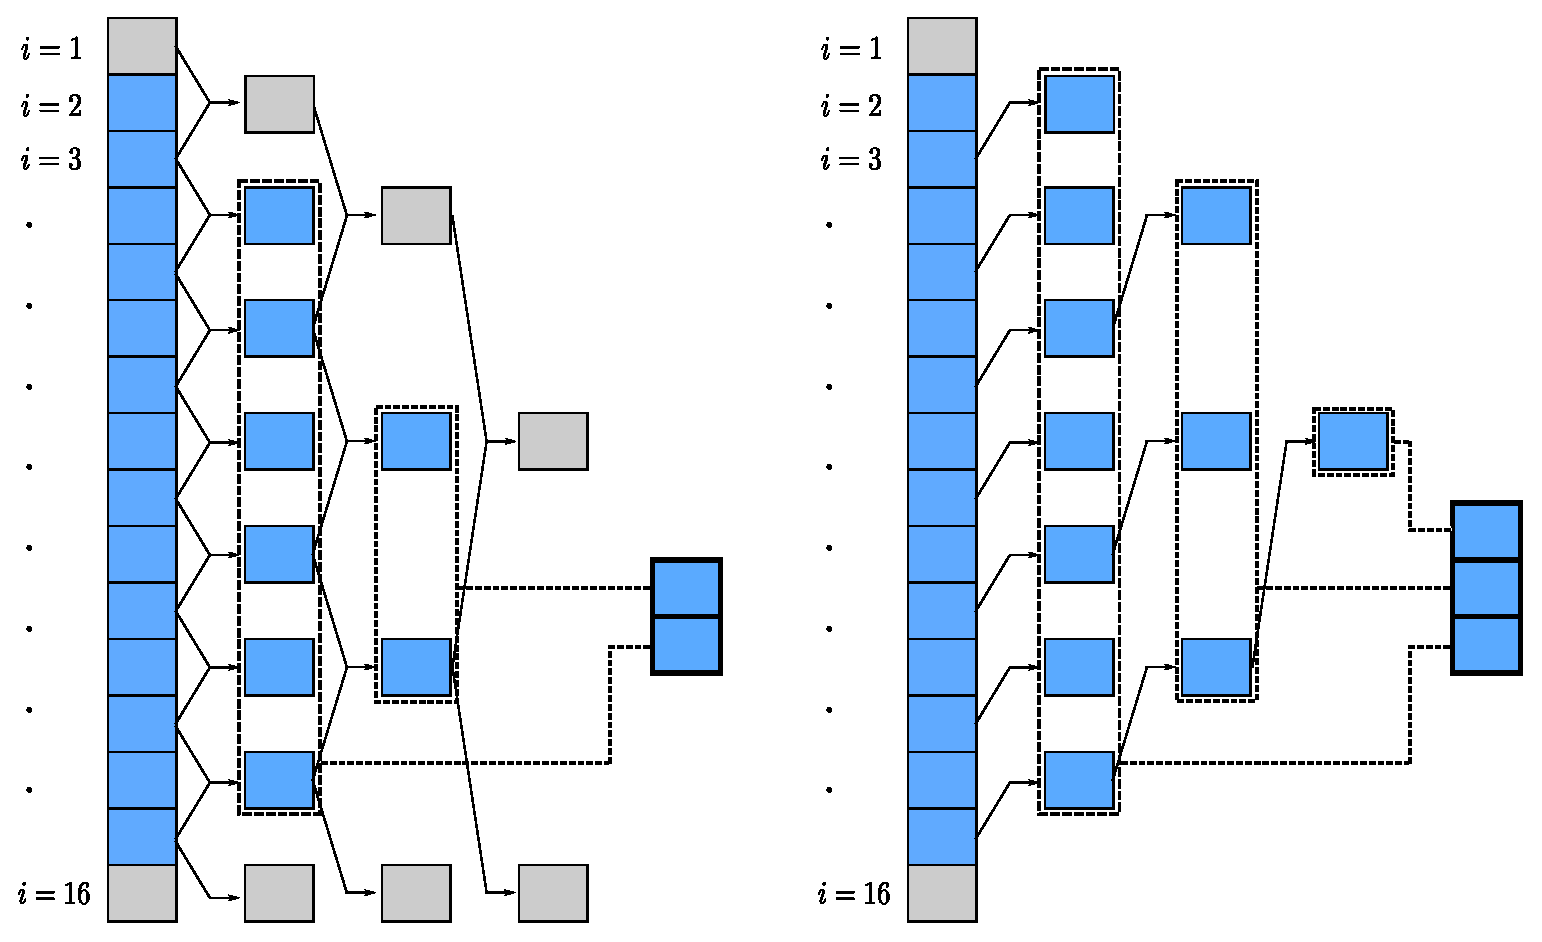
\includegraphics[height=200pt]{img/cyclic-reduction-boundaries.eps}
\end{center}
\caption{Indices affected by boundaries in cyclic reduction}
\label{fig:cyclic-reduction-boundaries}
\end{figure}

Precomputing the forward reduction coefficients
becomes especially effective for near-Toeplitz matrices.
At each reduction step,
the coefficients $a_i$, $b_i$, $c_i$, $k_{1,i}$ and $k_{2,i}$ 
are the same for all indices $i$,
except for indices ``polluted'' by the boundary conditions
(Figure \ref{fig:cyclic-reduction-boundaries}).
Further, a careful analysis of the equations
\ref{eqn:forward-reduction-1}-\ref{eqn:forward-reduction-3}
reveals that the following extra arrays are required
to store the coefficients at the boundaries: 

\begin{enumerate}
    \item The values of $b_1$ at each reduction step
    \item The values of $k_{1,1}$ at each reduction step
    \item The values of $k_{1,n}$ at each reduction step
    \item The values of $a_n$ and $b_n$ at the final reduction step
        (required for the 2-by-2 solve)
\end{enumerate}

This puts the total storage for precomputed coefficients
at $8(log_2(n) - 1)+2$.
For symmetric near-Toeplitz matrices,
$c_i = a_i$, and $k_{1,i} = k_{2,i}$ away from the boundaries,
reducing storage to $6(log_2(n) - 1)+2$.


%----------------------------------------------------------------------%

\section{Results: single GPU} \label{sec:results-single-gpu}

\begin{figure}[h!]
\begin{center}
\includegraphics[height=200pt]{fig/compare-solvers-K20.eps}
\end{center}
\label{fig:compare-solvers-K20}
\end{figure}

\begin{figure}[h!]
\begin{center}
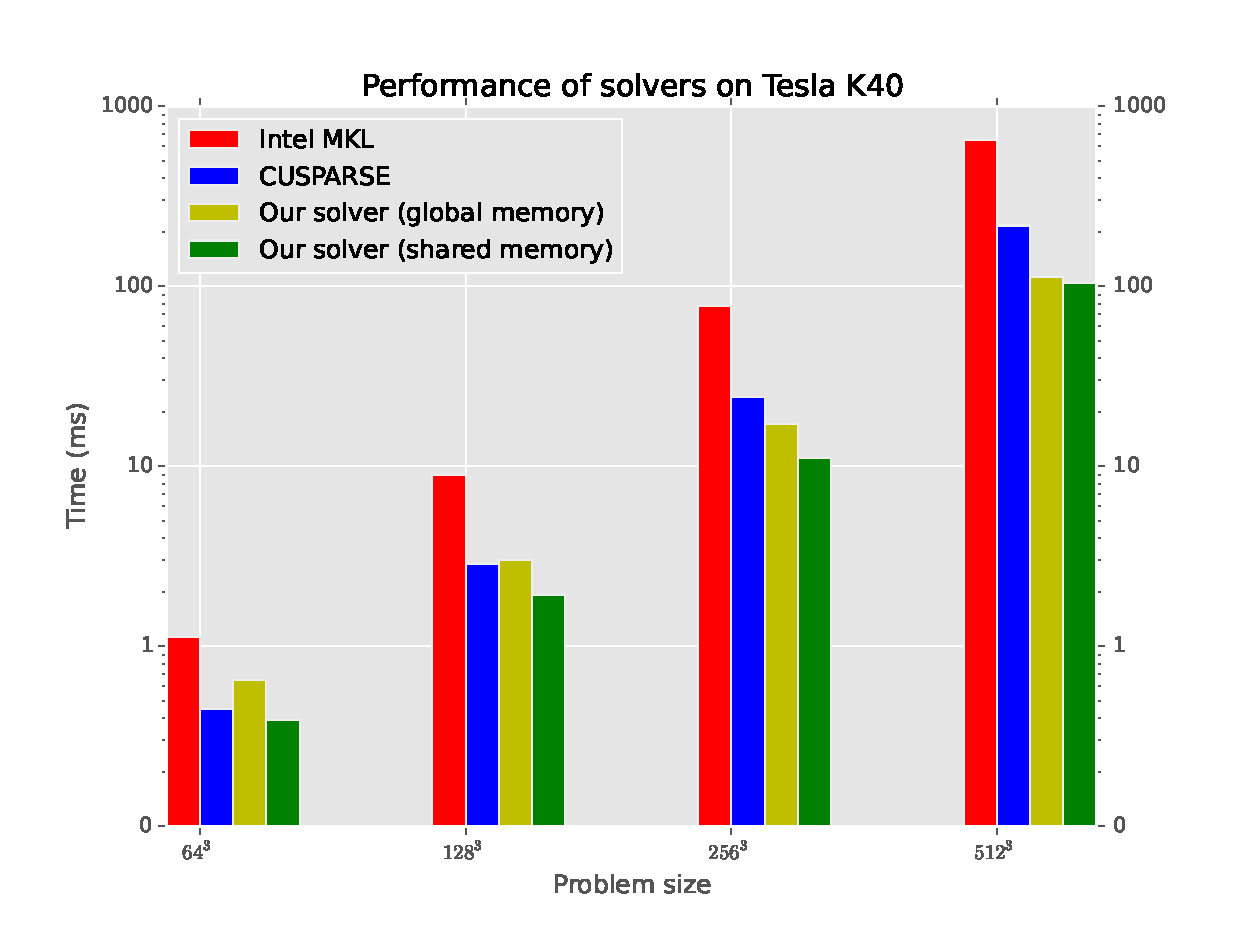
\includegraphics[height=200pt]{fig/compare-solvers-K40.eps}
\end{center}
\label{fig:compare-solvers-K40}
\end{figure}

\definecolor{light-gray}{gray}{0.95}
\begin{minted}[bgcolor=light-gray,linenos,fontsize=\footnotesize]{C++}
__global__ void forwardReduction( double *a_d, double *b_d,
        double *c_d, double *d_d, int n, int stride) {
    int tix = threadIdx.x;
    int i = (stride-1) + tix*stride;
    int offset = blockIdx.x*n;
    int stride;
    int m, n;
    double k1, k2;

    k1 = a_d[i]/b_d[i-stride/2];
    k2 = c_d[i]/b_d[i+stride/2];
    a_d[i] = -a_d[i-stride/2]*k1;
    b_d[i] = b_d[i] - c_d[i-stride/2]*k1 - a_d[i+stride/2]*k2;
    c_d[i] = -c_d[i+stride/2]*k2;
    d_d[offset+i] = (d_d[offset+i] - d_d[offset+i-stride/2]*k1 -
                        d_d[offset+i+stride/2]*k2);
}

__global__ void backwardSubstitution( double *a_d, double *b_d,
        double *c_d, double *d_d, int n, int stride) {
    int tix = threadIdx.x;
    int i = (stride/2-1) + tix*stride;
    int offset = blockIdx.x*n;
    d_d[offset+i] = (d_d[goffset+i] - a_d[i]*d_d[offset+i-stride/2] -
                        c_d[i]*d_d[offset+i+stride/2])/b_d[i];
}

\end{minted}

\begin{minted}[linenos,bgcolor=light-gray,fontsize=\footnotesize]{c++}

__global__ cyclicReduction(double *a_d, double *b_d, double *c_d,
    double *d_d, int n) {

    __shared__ double a_l[n];
    __shared__ double b_l[n];
    __shared__ double c_l[n];
    __shared__ double d_l[n];
    int i = threadIdx.x;
    int offset = blockIdx.x*n;
    int stride;

    /* Load coefficients and RHS into shared memory */
    a_l[i] = a_d[offset+i]; b_l[i] = b_d[offset+i];
    c_l[i] = c_d[offset+i]; d_l[i] = d_d[offset+i];

    /* Forward reduction */
    stride = 1;
    for (int k=0; k<log2(nx)-1; k++) {
        if (i < nx/stride) {
            k1 = a_l[i]/b_l[i-stride/2];
            k2 = c_l[i]/b_l[i+stride/2];
            a_l[i] = -a_l[i-stride/2]*k1;
            b_l[i] = b_l[i] - c_l[i-stride/2]*k1 - a_l[i+stride/2]*k2;
            c_l[i] = -c_l[i+stride/2]*k2;
            d_l[i] = d_l[i] - d_l[i-stride/2]*k1 - d_l[i+stride/2]*k2;
        }
        __syncthreads();
    }

    if (i == 0) {
        /* Solve the 2-by-2 system for d_l[n-1] & d_l[n/2-1] */
    }
    
    /* Backward substitution */
    stride = n;
    for (int k=0; k<log2(nx)-1; k++) {
        stride = stride/2;
        if (lix < nx/stride){
            d_l[i] = (d_l[i] - a_l[i]*d_l[i-stride/2] -
                        c_l[i]*d_l[i+stride/2])/b_l[i];
        }
        __syncthreads();
    }

    /* Load the solution from shared memory to global memory */
    d_d[offset+i] = d_l[i];
}

\end{minted}

\section*{References}

\bibliography{references}
\bibliographystyle{elsarticle-num}
\end{document}
